\subsection[Crowding distance]{\label{identificadorReferenciaCruzada}
Crowding distance}

\ \ There are several nearest-neighbor approaches that can be employed to evaluate the distribution of solutions and the crowding distance has proved to be one of the more eficient [2]. The crowding distance of a solution is de ned as the circumference of the rectangle de ned by its left and right neighbors, and infinity if there is no neighbor. Figure 2 illustrates the concept of crowding. Solutions with high crowding distance are considered better solutions, as they introduce more diversity in the population. In Figure 1 the solutions a and d belonging to the rank 1 in terms of non-dominance have the best score in terms of crowding. Then follows the solution b and then c. The rectangle associated with c is the smallest one [5]. NSGA-II uses crowding distance in its selection operator to keep a diverse front by making sure each member stays a crowding distance apart.
\begin{figure}[h!]
\begin{center}
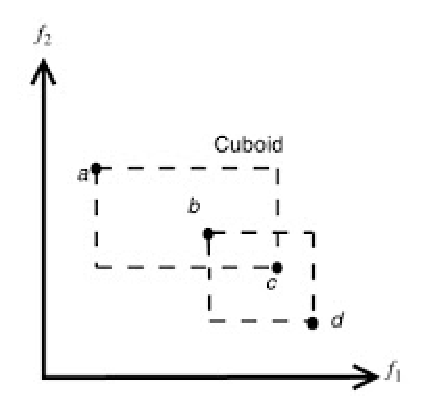
\includegraphics[width = 5cm] {./Graphics/Figure2.eps} 

\caption{Crowding distance [5]}
\end{center}
\end{figure}